\chapter{Methodologies}
\label{chap:methods}

This chapter illustrates the methodology used to approach the development process of this work.The application is divided into three main independent instances: gesture recognition, \gls{3d} trajectory detection and drone controller. First of all, the Section \ref{sec:handgestrec} to create a \gls{dnn} model to recognize hand gestures, followed by Section \ref{sec:getdata} and \ref{sec:model} which describes the type of data used for this purpose and how they are generated. After that, it will be shown how orientation and camera-hand distance has been estimated in Section \ref{sec:orientationestimation} and \ref{subsec:cam-hand} to detect a \gls{3d} trajectory. Next, there will be a focus on the drone controller in simulation and real. Section \ref{sec:pipeline} is concluded with a detailed explanation of the entire pipeline.

%pipeline
%mediapipe (poco perché già parlato tecnicamente)
%costruzione della rete neurale:
%	come devono essere i dati
%trasformazione matriciale
%algoritmo dei tre punti orientamento
%pitch
%yaw
%roll

\section{Hand Gesture Recognition}
\label{sec:handgestrec}
MediaPipe has a python implementation for its Hand Keypoints Detector. It returns $2.5D$ coordinates of $21$ hand landmarks (see Fig.\ref{fig:handland}), consisting of $x$, $y$, and relative $depth$. For this project the $depth$ coordinate of each hand landmark has been deleted to be estimated.

% https://towardsdatascience.com/control-dji-tello-drone-with-hand-gestures-b76bd1d4644f

\begin{figure}[H]
	\centering
	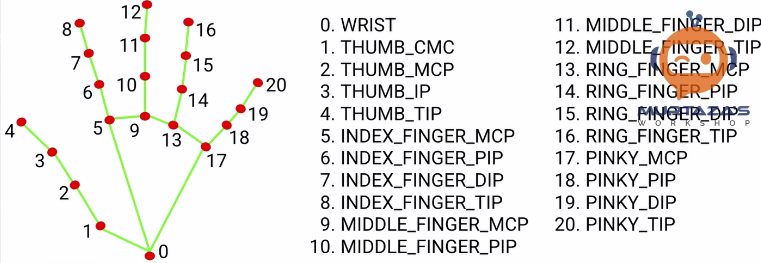
\includegraphics[width=.9\textwidth]{images/hand}
	\caption[Hand Landmarks.]{Image from the open MediaPipe repository.}
	\label{fig:handland}
\end{figure}

\noindent The coordinates of pixels in OpenCV follow a reference system $(x,y)$ in which the origin is in the top-left of each \gls{rgb} image frame, $x$ is column-wise and $y$ is row-wise on the computer screen. In order to normalize each point, the origin was converted from top-left to bottom-left. This resulted in the classic cartesian coordinate system. After that, the mean for $x$ and $y$ for each landmark was computed, converted in homogeneous coordinates and shifted them in order to match mean with origin. Note that shifting the data did not change how the data points are positioned relative to each other. Finally, each point has been scaled \gls{wrt} maximum distance from mean point to all other hand points. This normalization permits to compare same gesture at different positions from the camera, if same orientation. 

\subsection{Data Acquisition and Description}
\label{sec:getdata}
Following the normalization of the data, gestures that would allow to acquire a 3D trajectory and to interact directly with the drone have been thought. \\

\begin{figure}[H]
	\centering
	\includegraphics[width=1 \textwidth]{images/gestures}
	\caption[Full list of gestures.]{Full list of gestures that are available.}
	\label{fig:gestures}
\end{figure}

\noindent Below, there is the list of 10 gestures used in this project:
\begin{itemize}
	\item \texttt{backward}: this command allows the drone to go backwards;
	\item \texttt{detect}: this command allows the user to detect a \gls{3d} trajectory;
	\item \texttt{down}: this command allows the drone to go down;
	\item \texttt{forward}: this command allows the drone to go forward;
	\item \texttt{land}: this command allows the drone to land;
	\item \texttt{left}: this command allows the drone to go left;
	\item \texttt{ok}: this command allows the drone to conclude the \gls{3d} trajectory capturing and execute it;
	\item \texttt{right}: this command allows the drone to go right;
	\item \texttt{stop}: this command allows the drone to stop his movements;
	\item \texttt{up}: this command allows the drone to go up.
\end{itemize}

\noindent From the module that has been built there is the possibility to get data either from a webcam or from the drone camera. The dataset consists of $43$ columns: $42$ are the $21$ \gls{2d} points’ components, and the last one is the target. $1000$ examples were acquired, $100$ images for each gesture. In total, the dataset is composed of $43000$ elements. The python script to get data has also a restore in case of particular errors (e.g. if images are acquired from the drone, there could be problems due to overheating or low battery). Given the structure of the generation script, it is particularly easy to build a model with new gestures.

\subsection{Pearson Correlation}
\label{sec:pearsoncorr}
Correlation is a measure of the linear relationship of two or more variables. Through correlation, we can predict one variable from the other. The logic behind using correlation for feature selection is that the good variables are highly correlated with the target. Furthermore, variables should be correlated with the target but should be uncorrelated among themselves.

\noindent If two variables are correlated, one is predictable from the other. Therefore, if two features are correlated, the model only really needs one of them, as the second one does not add additional information. The Pearson Correlation through the heatmap plot has been used here.

\noindent A heatmap is a \gls{2d} graphical representation of data where the individual values that are contained in a matrix are represented as colors. The Seaborn python package allows the creation of annotated heatmaps which can be tweaked using Matplotlib tools as per the creator’s requirement.

\begin{figure}[H]
	\makebox[\textwidth]{
		\includegraphics[width=1.3 \textwidth]{images/corr}
	}
	\caption[Heatmap.]{Heatmap is really useful to display a general view of numerical data, not to extract specific data point. It represents the correlation matrix and it is done using Pearson correlation.}\label{fig:correlation}
\end{figure}

% https://stats.stackexchange.com/questions/392517/how-can-one-interpret-a-heat-map-plot
% https://www.analyticsvidhya.com/blog/2020/10/feature-selection-techniques-in-machine-learning/
% https://towardsdatascience.com/feature-selection-with-pandas-e3690ad8504b
\noindent Each square shows the correlation between the variables on each axis. Correlation ranges from $-1$ to $+1$. Values closer to zero imply weaker correlation (exact $0$ implying no correlation). A value closer to $1$ implies stronger positive correlation, that is as one increases so does the other and the closer to $1$ the stronger this relationship is. A correlation closer to $-1$ is similar, but instead of both increasing, one variable will decrease as the other increases. This is called negative correlation.

\noindent The diagonals are all $1$ because those squares are correlating each variable to itself (so it's a perfect correlation). The larger the number associated (in absolute) the higher the correlation between the two variables. The plot is also symmetrical to the diagonal since the same two variables are being paired together in those squares. This is the reason why just the lower matrix has been plotted.

\noindent Looking at the picture, it is possible to see that there is a high correlation between variables. Therefore, the correlation between features has been compared and one of two features that have an absolute correlation higher than $0.8$

\noindent After plotting the correlation matrix, an high level of correlation between each specified couple of variables has been found. Therefore, for those couples whose correlation where higher than $80\%$ one variable has been removed, since if two features are correlated, the model only needs one as the second does not bring additional information. 

\begin{figure}[H]
	\centering
	\includegraphics[width=1\textwidth]{images/featuresel}
	\caption[Feature Selection: Feature Vs Feature.]{Feature Selection: Feature Vs Feature.}
	\label{fig:featuresel}
\end{figure}

\noindent Note: a better version could be used, setting an absolute value, saying $0.5$ as the threshold for selecting the variables. If the predictor variables are correlated among themselves, the variable which has a lower correlation coefficient value with the target variable can be dropped. High results are gained just finding that if the predictor variables are correlated among themselves then one of them should be dropped. After this, features were selected, dropping columns that were highly correlated going from 42 to 9 variables. The final features given by Pearson correlation are: 

\noindent Below, there is the list of 10 gestures used in this project:
\begin{itemize}
	\item \texttt{WRIST\_X};
	\item \texttt{WRIST\_Y};
	\item \texttt{THUMB\_CMC\_X};
	\item \texttt{INDEX\_FINGER\_MCP\_Y};
	\item \texttt{INDEX\_FINGER\_PIP\_Y};
	\item \texttt{MIDDLE\_FINGER\_MCP\_X};
	\item \texttt{MIDDLE\_FINGER\_PIP\_X};
	\item \texttt{MIDDLE\_FINGER\_DIP\_X};
	\item \texttt{RING\_FINGER\_DIP\_Y}.
\end{itemize}

\subsection{PCA}
\label{sec:pca}
% https://www.reneshbedre.com/blog/principal-component-analysis.html#pca-interpretation
\gls{pca} is a classical multivariate (unsupervised machine learning) non-parametric dimensionality reduction method that used to interpret the variation in high-dimensional interrelated dataset (dataset with a large number of variables). \gls{pca} reduces the high-dimensional interrelated data to low-dimension by linearly transforming the old variable into a new set of uncorrelated variables called principal component (\gls{pc}) while retaining the most possible variation. The first component has the largest variance followed by the second component and so on. The first few components retain most of the variation, which is easy to visualize and summarise the feature of original high-dimensional datasets in low-dimensional space. \gls{pca} helps to assess which original samples are similar and different from each other. \\

\begin{figure}[htbp]
	\makebox[\textwidth]{
		\includegraphics[width=1.3 \textwidth]{images/bipca}
	}
	\caption[\gls{pca} - Biplot.]{After dimensionality reduction, there usually is not a particular meaning assigned to each principal component. The new components are just the two main dimensions of variation.}\label{fig:bipca}
\end{figure}

\noindent As \gls{pca} is based on the correlation of the variables, it usually requires a large sample size for the reliable output. The sample size can be given as the absolute numbers or as subjects to variable ratios. The minimum absolute sample size of $100$ or at least $10$ or $5$ times to the number of variables is recommended for \gls{pca}. On other hand, Comrey and Lee’s (1992) have a provided sample size scale and suggested the sample size of $300$ is good and over $1000$ is excellent. \\

\noindent As the number of \glspl{pc} is equal to the number of original variables, only the \glspl{pc} should be kept, which explain the most variance ($70-95\%$) to make the interpretation easier. The more \glspl{pc} that explains most variation in the original data are included, the better the \gls{pca} model will be. This is highly subjective and based on the user interpretation \cite[]{cangelosi2007component}. \\

\noindent For a lot of machine learning applications, it helps to be able to visualize the dataset. Visualizing two or three dimensional data is not that challenging. However, things are different when the dimension is above four.\gls{pca} can be used to reduce that $n$ dimensional data into two or three dimensions so that data can be plotted and understood. For this reason it is possible to say that \gls{pca} can also be used for Data Visualization. \\

\noindent \gls{pca} is effected by scale so scaling the features is needed in the data before applying \gls{pca}. In Sklearn Framework using StandardScaler() function helps to standardize the dataset’s features onto unit scale ($mean = 0$ and $variance = 1$), which is a requirement for the optimal performance of many machine learning algorithms. An alternative standardization is scaling features to lie between a given minimum and maximum value, often between zero and one, or so that the maximum absolute value of each feature is scaled to unit size. This can be achieved using MinMaxScaler or MaxAbsScaler function, respectively. A Problem about StandardScaler is when there is new data, and this cannot be scaled as the dataset used to build the \gls{ml} model.MinMaxScaler function has been chosen. \\

\noindent Biplots (see Fig. \ref{fig:bipca}) are useful to visualize the relationships between variables and observations. The original data has $n$ columns and the original data which is $m$ dimensional into \gls{2d} is projected (where $m$ is the number of rows, in other words, the sample number of the dataset). From the biplot and loadings plot, it is possible to see that a lot of variables are highly associated and forms cluster. If the variables are highly associated, the angle between the variable vectors should be as small as possible in the biplot. The length of PCs in biplot refers to the amount of variance contributed by the \glspl{pc}. The longer the length of \gls{pc}, the higher the variance contributed and well represented in space. The first two \glspl{pc} contribute $~70,43\%$ of the total variation in the dataset. \\

\noindent Scree plot (see Fig. \ref{fig:screeplot}) is another graphical technique useful in \glspl{pc} retention. The \glspl{pc} where there is a sharp change in the slope of the line connecting adjacent \glspl{pc} shuold be kept. Only the $6$ \gls{pc} have been taken because they describe around the $93\%$ of the total variation in the dataset .

\begin{figure}[H]
	\centering
	\includegraphics[width=.8\textwidth]{images/screeplot}
	\caption[Scree plot.]{Scree plot.}
	\label{fig:screeplot}
\end{figure}

\subsection{Model}
\label{sec:model}
For classification tasks there are a variety of different estimators/models from which it is possible to choose. In the end, DNNClassifier from Tensorflow Framework has been used, with two hidden layers composed of $30$ and $10$ neurons each. Input layer is composed of $42$ elements and the output layer of 10 classes (see Fig. \ref{fig:handarch}). The model must choose among ten classes, so the gestures descripted in \ref{sec:getdata}. The activation function is the Leaky ReLU and Adam the optimizer with learning rate $0.1$, decay steps $10000$ and decay rate $0.96$. About the steps, for the training phase $3000$ as value has been chosen. Loss is calculated by using softmax cross entropy.

% https://github.com/ashishpatel26/Tools-to-Design-or-Visualize-Architecture-of-Neural-Network
% http://alexlenail.me/NN-SVG/index.html

\begin{figure}[H]
	\makebox[\textwidth]{
		\includegraphics[width=1.1 \textwidth]{images/net}
	}
	\caption[Hand gesture reconognition \gls{nn}.] {\gls{dnn} image of the hand gesture recognition, generated by NNSVG\footnote{\url{http://alexlenail.me/NN-SVG/index.html}}. This is the specific case when all the $42$ variables were given as input.}
	\label{fig:handarch}
\end{figure}

\noindent Three models were genearated: one using the entire dataset, one using just only the selected features and finally one using \gls{pca}. Because of such a simple structure, high accuracy was reached for all of them. It is not required to retrain the model for each gesture in different illumination (or building a convolutional neural network), because MediaPipe takes over all the detection work.

\section{3D trajectory detection}
\label{sec:3dtraj}
Trajectories will be detected using the detect gesture (see Fig. \ref{fig:gestures} (c)). The experiments about orientation estimation will be executed only on that gesture. 

\subsection{Orientation estimation}
\label{sec:orientationestimation}

\begin{figure}[H]
	\centering
	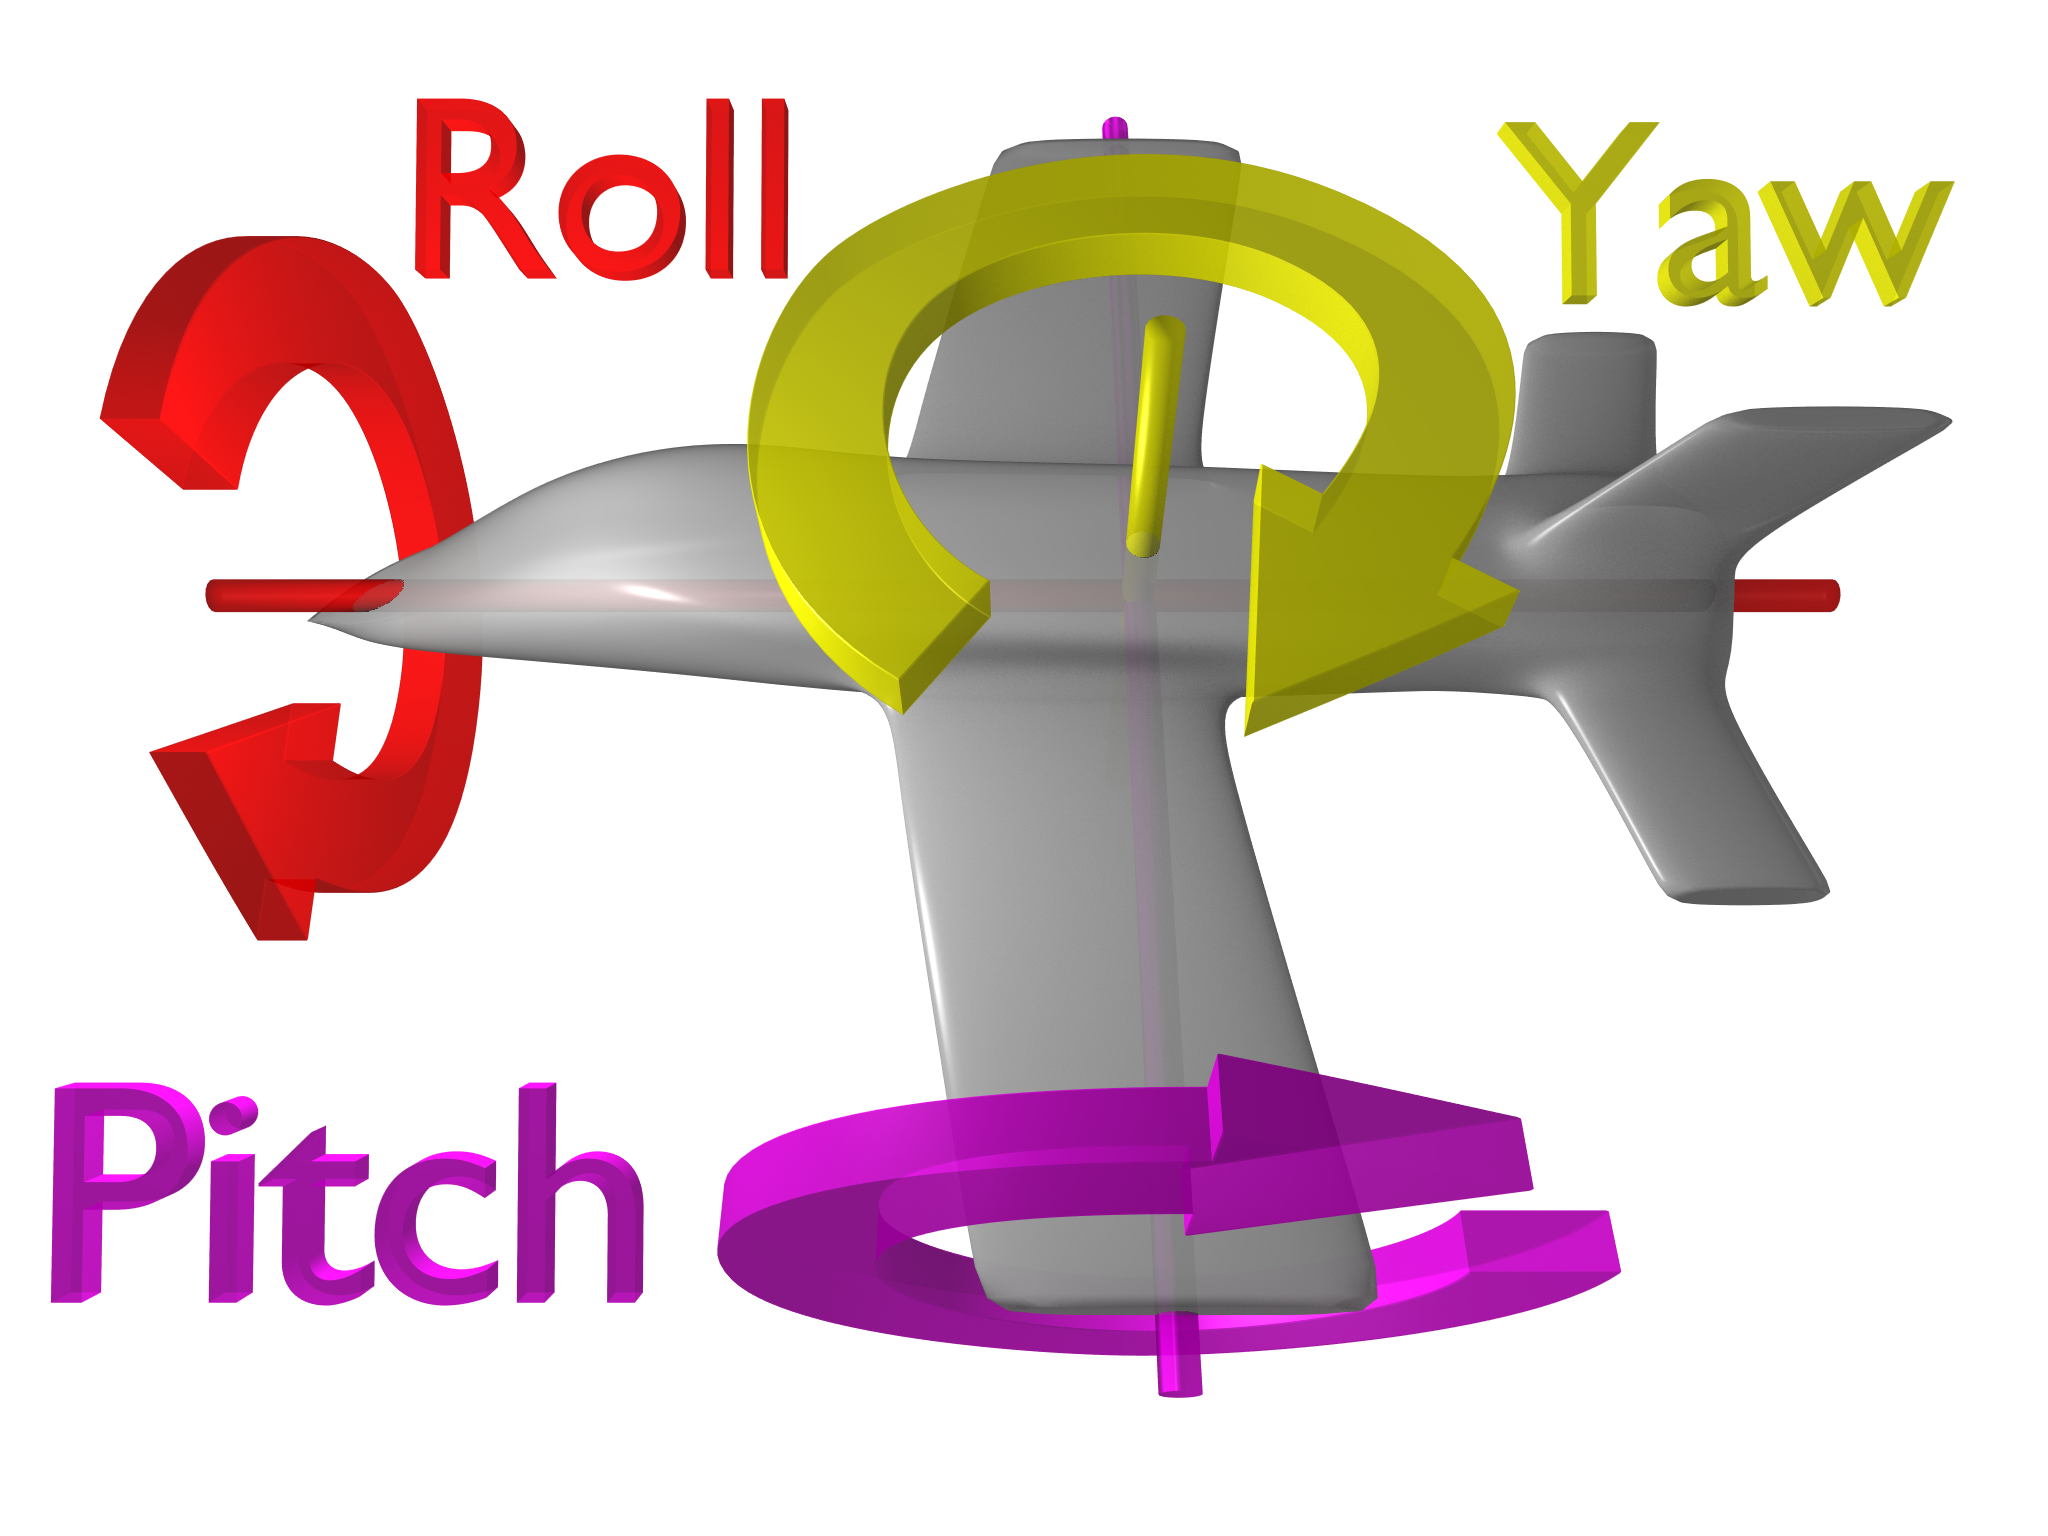
\includegraphics[width=.6\textwidth]{images/orientation}
	\caption[Aircraft principal axes.]{Aircraft principal axes.}
	\label{fig:orientation}
\end{figure}

% Note that yaw and pitch orientation estimates are made after the hand points are normalized, while roll is computed at the time of normalization, as described in. The normalization in this phase occurs by first of all making the translation so that the origin of the axes matches the midpoint of the hand, then all the points of the hand are scaled so that the maximum distance between them and the origin has a value of 1. Finally we rotate the hand with respect to the roll value computed during the normalization phase.
In the following section, the methods used to perform yaw, roll and pitch measurements starting from the pixels of the image captured with a camera will be discussed. Note that yaw and pitch orientation estimates are made after the hand points are normalized, while roll is computed at the time of normalization, as described in. The normalization in this phase occurs by first of all making the translation so that the origin of the axes matches the midpoint of the hand, then all the points of the hand are scaled so that the maximum distance between them and the origin has a value of 1. Finally, the hand is rotated \gls{wrt} the roll the value computed during the normalization phase.

\subsubsection{Turning and orientations}
\label{subsec:orientationtest}

In order to find a value for the yaw, it is needed to understand how to determine whether three points form a left-hand turn. This can be done by an orientation test, which is fundamental to many algorithms in computational geometry \cite[]{CMSC75428:online}. Given an ordered triple of points $\langle p, q, r \rangle$ in the plane, they have a positive orientation if they define a counterclockwise oriented triangle (see Fig. \ref{fig:orientationtest} (a)), negative orientation if they define a clockwise oriented triangle (see Fig. \ref{fig:orientationtest} (b)), and zero orientation if they are collinear, which includes as well the case where two or more of the points are identical (see Fig. \ref{fig:orientationtest} (c)). It is important to take care about the fact that the orientation depends on the order in which the points are given.

\begin{figure}[H]
	\centering
	\includegraphics[width=.9\textwidth]{images/orientationtest}
	\caption[Orientation test.]{Orientations of the ordered triple (p, q, r).}
	\label{fig:orientationtest}
\end{figure}

\noindent Orientation is formally defined as the sign of the determinant of the points given in homogeneous coordinates, that is, by prepending a 1 to each coordinate. For example, in the plane see Eq. \ref{eq:orientationtest}

% https://jasonwarta.github.io/latex-matrix/ 
\begin{Equation}[!htb]
	\centering
	\begin{equation} \label{eq:orientationtest}
		Orient(p,q,r) = det
		\begin{pmatrix}
			1 & p_x & p_y \\
			1 & q_x & q_y \\
			1 & r_x & r_y 
		\end{pmatrix}
		\end{equation}
	\caption[Orientation test.]{Thus orientation generalizes the familiar \gls{1d} binary relations $<, =, >$.}
\end{Equation}

\noindent The sign of the orientation of an ordered triple is unchanged if the points are translated, rotated, or scaled (by a positive scale factor). In general, applying any affine transformation to the point alters the sign of the orientation according to the sign of the determinant of the matrix used in the transformation. \\

\noindent If points belonging to the same reference system are considered and the orientation test is computed then it is possible to get information on how much the points are crushed together. 

\subsubsection{Roll estimation}
\label{subsec:roll}
To estimate the roll, the angle generated by the vertical axis passing over the wrist and the tip of the middle finger has been found (see fig. \ref{fig:handland}).

\subsubsection{Yaw estimation}
\label{subsec:yaw}
First of all, it is necessary to fix a hand to estimate the yaw. This project will be carried on the left-hand, so each comment will be in that direction. Despite this, the same can be said for the right hand. Then, the orientation test (see Eq. \ref{eq:orientationtest}) of three points $\langle p, q, r \rangle$ is computed. As already said, the order here is important to find the direction of orientation, therefore to know if the left-hand points left or right and with which intensity. Empirically, if $roll < \ang{-5}$ or $roll > \ang{+5}$ it is better to consider $p=$ index\_finger\_mcp, $q=$ index\_finger\_pip and $r=$ index\_finger\_dip. Otherwise, if $\ang{-5} < roll < \ang{+5}$ results are good if $p=$ middle\_finger\_mcp, $q=$ middle\_finger\_pip and $r=$ middle\_finger\_dip. These hand points were chosen because they scale quite well with hand orientation. \\

\noindent The value of the orientation test is raised to the second power, in order to be more stable around \ang{0}. Then, it is divided by $1666$, a number computed empirically to bring the results obtained from the orientation test to the range of \ang{-90} to \ang{+90}. Since the quadratic form was used, this value will be very huge if greater than \ang{+90} or smaller than \ang{-90}, for this reason the part the exceeds has been reduced to be just the $10\%$ of it.

\subsubsection{Pitch estimation}
\label{subsec:pitch}
To compute pitch estimation, the middle point $m$ between index\_finger\_mcp and index\_finger\_pip were copmuted and then the difference between $m$ and the thumb\_tip \gls{wrt} vertical axis was done (see fig. \ref{fig:handland}). As for yaw estimation, the value obtained is elevated to the second power, in order to be more stable around \ang{0}. Then, the result was divided by $31$ (empirically computed), to bring the results to the range of \ang{-90} to \ang{90}. Since the quadratic form was used, if the value is greater than \ang{90} or smaller than \ang{-90} the results tends to be really big, therefore the part the exceeds has been reduced to be just the 10\% of it.

\subsection{Camera-hand distance estimation}
\label{subsec:cam-hand}
%Nella fase iniziale di identificazione di una traiettoria 3d, il palmo della mano è perpendicolare rispetto al raggio d'azione dalla lente della fotocamera. La mano all'inizio è ferma e nell'immagine acquisita la stessa mano possiede una certa area h. Se consideriamo il punto centrale p della mano come la distanza media tra tutti i punti di riferimento della mano allora tale punto p possiamo considerarlo l'origine di un sistema di riferimento cartesiano ortogonale a tre assi. 
%
%Se volessimo trattare la mano come un punto materiale, cioè che non cambia il suo orientamento nello spazio, allora catturare tutti i punti medi della mano e confrontare le aree della mano per stimare le profondità nel corso del tempo t significa ottenere quei punti che identificano una traiettoria 3d. 
%
%Se però volessimo trattare la mano come un corpo, e quindi stimare anche il suo orientamento nello spazio allora le cose si complicano. Infatti, seppur comunque riusciremmo a identificare lo spostamento bidimensionale della mano, in termini di altezza e larghezza, come se trattassimo la mano come un punto materiale, invece non potremmo più confrontare le aree della mano perché queste possono essere alterate a causa dell'orientamento della mano assunta in un certo istante di tempo. Ecco perchè abbiamo di stimare l'orientamento della mano nello spazio, perché così possiamo proiettare i punti che descrivono la mano in modo che la mano sia perpendicolare rispetto al raggio d'azione della lente della fotocamera, quindi a ricondurci al caso precedente, ovvero confrontare le aree della mano per stimare la profondità.

In the initial phase of identifying a \gls{3d} trajectory, the palm of the hand is perpendicular to the range of action from the camera lens. At the beginning, the hand is still and in the acquired image the same hand has a certain area $h$. If the central point $p$ of the hand is considered as the average distance between all the reference points of the hand, then $p$ can be considered the origin of an orthogonal three-axis Cartesian reference system.

\noindent If the hand was treated as a material point, i.e. that does not change its orientation in space, then capturing all the midpoints of the hand and comparing the areas of the hand to estimate the depths over time t means obtaining those points that identify a trajectory \gls{3d}.

\noindent However, if the hand was treated as a body, and therefore also estimate its orientation in space, then things get complicated. In fact, although identifying \gls{2d} hand displacement, in terms of height and width, would be possible as if the hand was being treated as a material point, instead the areas of the hand could not be compared because these can be altered due to the orientation of the hand. This is why the orientation of the hand has to be estimated in space, because in this way the points that describe the first hand detected can be projected. Thus, bringing it back to the previous case, comparing areas of the hand to estimate depth. \\


%Quindi dopo aver rilevato il primo gesto, è stato calcolato il punto medio p e tutti punti della mano sono stati traslati in modo tale che il punto medio p diventi l'origine della mano. Notare che, a differenza di come è stato fatto per normalizzare i dati come ingresso per la rete neurale, qui non scaliamo i punti rispetto la massima distanza tra punto medio e tutti gli altri punti della mano. Non lo facciamo perché non vogliamo perdere l'informazione dello scaling. Anche tutti i gesti sucessivi (sempre riferiti al gesto del "detect") con possibile orientamento diverso vengono catturati ed eseguito lo stesso processo di normalizzazione. A ogni frame computiamo il valore della profondità confrontando la prima mano acqusita con quella in corso. Nello specifico, ai punti che definiscono la prima mano acquisita attuiamo una trasformazione matricale: una rotazione 3D lungo i 3 assi sfruttando le stime dello yaw, roll e pitch calcolare precedentmente

\noindent So after detecting the first gesture, the midpoint $p$ was calculated and all points of the hand were translated in such a way that the midpoint $p$ becomes the origin of the hand. Note that, unlike how it was done to normalize the data as an input to the \gls{nn}, here the points were not scaled \gls{wrt} the maximum distance between the midpoint and all other points of the hand. This is not done to lose the scaling information. Also all subsequent gestures (always referring to the "detect" gesture) with possible different orientation are captured and performed the same normalization process. At each frame the depth value is calculated by comparing the first hand acquired with the one in progress. Specifically, at the points that define the first hand acquired a matrix transformation was implemented: a \gls{3d} rotation along the three axes using the estimates of the yaw, roll and pitch calculated previously (see \ref{sec:orientationestimation}).

\noindent A rotation matrix rotates an object about one of the three coordinate axes or any arbitrary vector. The rotation matrix is more complex than the scaling and translation matrix since the whole $3x3$ upper-left matrix is needed to express complex rotations. It is common to specify arbitrary rotations with a sequence of simpler ones each along with one of the three cardinal axes. In each case, the rotation is through an angle, about the given axis. As in \ref{eq:rotx}, \ref{eq:roty} and \ref{eq:rotz}, the three matrices $R_Z$, $R_Y$ and $R_X$ represent transformations that rotate points through an angle $\theta$ in radians about the coordinate origin. Borrowing aviation terminology, these rotations will be referred to as yaw, pitch, and roll \cite[]{Yawpitch48:online}.

% http://planning.cs.uiuc.edu/node102.html
\begin{Equation}[!htb]
	\centering
	\begin{equation} \label{eq:rotx}
	R_Z(\alpha) =
        \begin{pmatrix}
            cos\alpha & -sin\alpha & 0 & 0 \\
            sin\alpha & cos\alpha & 0 & 0 \\
            0 & 0 & 0 & 0 \\
            0 & 0 & 0 & 1 
        \end{pmatrix}
	\end{equation}
	\caption[Z-Rotation Matrix in homogeneous coordinates.]{Z-Rotation Matrix in homogeneous coordinates. A yaw is a counterclockwise rotation of $\alpha$ about the z-axis.}
\end{Equation}

\begin{Equation}[!htb]
	\centering
	\begin{equation} \label{eq:roty}
	R_Y(\beta) =
        \begin{pmatrix}
            cos\beta & 0 & sin\beta & 0 \\
            0 & 1 & 0 & 0 \\
            -sin\beta & 0 & cos\beta & 0 \\
            0 & 0 & 0 & 1 
        \end{pmatrix}
	\end{equation}
	\caption[Y-Rotation Matrix in homogeneous coordinates.]{Y-Rotation Matrix in homogeneous coordinates. A pitch is a counterclockwise rotation of $\beta$ about the y-axis.}
\end{Equation}

\begin{Equation}[!htb]
	\centering
	\begin{equation} \label{eq:rotz}
	R_X(\gamma) =
        \begin{pmatrix}
            1 & 0 & 0 & 0 \\
            0 & cos\gamma & -sin\gamma & 0 \\
            0 & sin\gamma & cos\gamma & 0 \\
            0 & 0 & 0 & 1 
        \end{pmatrix}
	\end{equation}
	\caption[X-Rotation Matrix in homogeneous coordinates.]{X-Rotation Matrix in homogeneous coordinates. A roll is a counterclockwise rotation of $\gamma$ about the x-axis.}
\end{Equation} 

\noindent It must be further defined whether positive angles perform a clockwise (CW) or counterclockwise (CCW) rotation around an axis \gls{wrt} a specification of the orientation of the axis. Here, positive rotation angles cause a counterclockwise rotation about an axis as one looks inward from a point on the positive axis toward the origin. This is commonly the case for right-handed coordinate systems. Note that transformation matrices containing only rotations and translations are examples of rigid-body (solid-body) transformations, which do not alter the size or shape of an object. The yaw, pitch, and roll rotations can be used to place a \gls{3d} body in any orientation. A single rotation matrix $R$ can be formed by multiplying the yaw, pitch and roll rotation matrices (see Eq. \ref{eq:genrot}).

\begin{Equation}[H]
	\centering
	\begin{equation}
	    \begin{gathered}
    		R(\alpha, \beta, \gamma) = R_X(\alpha) \cdot R_Y(\gamma) \cdot R_Z(\beta)
    		= \\
            \begin{pmatrix}
                cos\alpha \, cos\beta & cos\alpha \, sin\beta \, sin\gamma-sin\alpha \, cos\gamma & cos\alpha \, sin\beta \, cos\gamma +sin\alpha \, sin\beta & 0 \\
                sin\alpha \, cos\beta & sin\alpha \, sin\beta \, sin\gamma +cos\alpha \, cos\gamma & sin\alpha \, sin\beta \, cos\gamma -cos\alpha \, sin\gamma & 0 \\
                -sin\beta & cos\beta \, sin\gamma & cos\beta \, cos\gamma & 0 \\
                0 & 0 & 0 & 1 
            \end{pmatrix}
        \end{gathered}
	\end{equation}
	\caption[General Rotation.]{General rotation matrix, used to perform a rotation in Euclidean space.}
	\label{eq:genrot}
\end{Equation}

\noindent It is important to state that $R(\alpha, \beta, \gamma)$ performs the roll first, then the pitch, and finally the yaw. If the order of these operations is changed, a different rotation matrix would result. 

\noindent Instead of calculating the area of the hand, the mean of the sums of the distances between the hand midpoint p and all other reference hand landmark was calculated to have a more robust metric. After having performed this last operation both on all the points of the current hand and on the first hand transformed with the general matrix, we finally made the difference between the first and the second value obtained previously has been finally made. In this way, it is possible obtain a depth estimate of the hand (which is performing the detecting gesture) even if it is oriented in space.

\subsection{Errors}
\label{sec:errors}
\noindent The trajectory acquired in the previous phase is pure and for this reason it presents some noise. This noise is conditioned by a series of dependent events. In fact, at the base of everything, there is the error given by the precision with which the "detect" gesture is detected by the Mediapipe solution. In fact, although the classifier has a high level of accuracy, being a solution in real time and designed to work on smartphone devices, it has limits dictated by the computational components that means that the classifier cannot have an architecture that is too complex, and therefore this translates that in some frames the hand landmark is not correctly captured. Above this first level of error, there are three other incorrectness which are connected to the estimates of the orientation components. These inaccuracy are the ones bring more problems to the whole system. Finally, the error that describes the correctness with which the depth of the points of the trajectory was estimated was found. The latter represents the inaccuracy that reports the greatest inaccuracy to the system because it is a combination of the four errors described above. \\

\noindent In the idea of a practical application, the acquisition of trajectories can be done from a computer webcam or from a mobile phone camera. In this case it is possible to speak of acquisition with a fixed camera in space. Another level of application could be that of direct interaction with the drone, therefore with a potentially moving camera. Although the drone can be programmed to make it remain stable in one point in space, it does not imply that it is also capable of withstanding atmospheric agents, specifically the wind. In the latter use case, an additional level of error is added to the base of the whole system. it is easy to understand that the error is not something negligible and that it must necessarily be managed.

\subsection{Smoothing}
\label{sec:smoothing}

In the different areas of science, smoothing a dataset means creating an approximating function that attempts to capture important patterns in the data, while leaving out noise or other fine-scale structures/rapid phenomena. In smoothing, because of noise, the data points of a signal are modified so individual points higher than the adjacent points are reduced, and points that are lower than the adjacent points are increased leading to a smoother signal. Smoothing may be used in two important ways that can aid in data analysis by being able to extract more information from the data as long as the assumption of smoothing is reasonable and able to provide analyses that are both flexible and robust. \\

% https://statisticaloddsandends.wordpress.com/2019/10/03/generalized-ridge-regression-and-smoothing-splines/

\noindent The trajectory $g(x, y, z)$ acquired in a certain time $t$, two different smoothing algorithms have been computed on it: spline and ridge regression.
%https://blog.finxter.com/fitting-data-with-scipys-univariatespline-and-lsqunivariatespline/
Splines are mathematical functions that describe an ensemble of polynomials which are interconnected with each other in specific points called the knots of the spline. They are used to interpolate a set of data points with a function that shows a continuity among the considered range; this also means that the splines will generate a smooth function, which avoids abrupt changes in slope. Compared to the more classical fitting methods, the main advantage of splines is that the polynomial equation is not the same throughout the whole range of data points. Instead, the fitting function can change from one interval to the subsequent one, allowing for fitting and interpolation of very complicated point distributions. \\

\noindent One of the main characteristics of splines is their continuity; they are continuous along the entire interval in which they are defined; this allows for the generation of a smooth curve, that fit our set of data points. One of the main advantages of using splines for fitting problems, instead of single polynomials, is the possibility of using lower degree polynomial functions to describe very complicated functions. Indeed, if a single polynomial function was needed, the degree of the polynomial usually would increase with the complexity of the function that has to be described; increasing the degree of the fitting polynomial could introduce the Runge's phenomenon problem (see Fig \ref{fig:runge}), in which oscillation can occur between points when interpolating using high-degree polynomials. \\

\begin{figure}[H]
	\centering
	\includegraphics[width=.8\textwidth]{images/runge.png}
	\caption[Runge's phenomenon problem.]{Runge's phenomenon problem.}
	\label{fig:runge}
\end{figure}

\noindent From the Scipy package there is the function UnivariateSpline() to calculate \gls{1d} smoothing spline $y = spl(x)$ of degree $k$ to the provided $x, y$ data. One of the most important parameters is $k$, which refers to the degree of the polynomials that define the spline segments and it varies between one and five (e.g. $k = 3$ is a cubic spline). Increasing the degree of the polynomials allows a better fitting of more complicated functions, but in order not to introduce artifacts in the fit, the best practice is to use the lower degree that allows for the better fitting procedure. Another relevant parameter is $s$, it is a float number which defines the smoothing factor, which directly affects the number of knots present in the spline. Once a specific value of $s$ is fixed, the number of knots will be increased until the difference between the value of the original data points and their respective datapoints along the spline is less than the value of $s$.

\begin{figure}[H]
	\centering
	\includegraphics[width=.8\textwidth]{images/spline1d.png}
	\caption[Smoothing spline 1D.]{Smoothing spline \gls{1d}}
	\label{fig:spline1d}
\end{figure}

% https://machinelearningmastery.com/ridge-regression-with-python/
\noindent Another technique of data fitting is Linear regression. Linear regression refers to a model that assumes a linear relationship between input variables and the target variable. With a single input variable, this relationship is a line, and in higher dimensions it can be thought of as a hyperplane that connects the input variables to the target variable. The coefficients of the model are found via an optimization process that seeks to minimize the \gls{sse} between the predictions and the expected target values. A problem with linear regression is that estimated coefficients of the model can become large, making the model sensitive to inputs and possibly unstable, especially for problems with few samples or less samples than input variables. \\

\noindent One approach to address the stability of regression models is to change the loss function to include additional costs for a model that has large coefficients. Linear regression models that use these modified loss functions during training are referred to collectively as penalized linear regression. One popular penalty is to penalize a model based on the sum of the squared coefficient values (beta). This is called an $L2$ penalty. The effect of this penalty is that the parameter estimates are only allowed to become large if there is a proportional reduction in \gls{sse}. In effect, this method shrinks the estimates towards $0$ as the lambda penalty becomes large (these techniques are sometimes called “shrinkage methods”). This penalty can be added to the cost function for linear regression and is referred to as Tikhonov regularization or Ridge Regression more generally. A hyperparameter is used called “lambda” that controls the weighting of the penalty to the loss function. A value of $1$ will fully weight the penalty; a value of $0$ excludes the penalty. Very small values of lambda, such as $1e-3$ or smaller are common. From the Scipy package there is the function Ridge() to solve a regression model where the loss function is the linear least squares function and regularization is given by the $L2$-norm.

\begin{figure}[H]
	\centering
	\includegraphics[width=1\textwidth]{images/ridge1d.png}
	\caption[Ridge regression 1D.]{Sample fits on a high degree polynomial function with some random noise. As alpha grows larger the model will overgeneralize (under-fit), while at lower values of alpha, the model may be too specific (overfit).}
	\label{fig:ridge1d}
\end{figure}

\noindent Another way to see the effectiveness of this method is plot the ridge coefficients as a function of the regularization (see Fig. \ref{pltridgecoeff} . Each color represents a different feature of the coefficient vector, and this is displayed as a function of the regularization parameter. A slight change in the target variable can cause huge variances in the calculated weights. In such cases, it is useful to set a certain regularization (lambda) to reduce this variation (noise). When lambda is very large, the regularization effect dominates the squared loss function and the coefficients tend to zero. At the end of the path, as alpha tends toward zero and the solution tends towards the ordinary least squares, coefficients exhibit big oscillations. In practise it is necessary to tune alpha in such a way that a balance is maintained between both.

\begin{figure}[H]
	\begin{minipage}{\textwidth}
		\centering
		\includegraphics[width=.7\textwidth]{images/pltridgecoeff}
		\caption[Ridge coefficients as a function of the regularization.]{Ridge coefficients as a function of the regularization, image from scikit-learn website \footnote{https://scikit-learn.org/stable/auto\_examples/linear\_model/plot\_ridge\_path.html}.}
		\label{fig:pltridgecoeff}
	\end{minipage}
\end{figure}

\noindent At the implementation level, given the trajectory $g(x, y, z)$ the cumulative sum of distances between each pair of adjacent points was calculated. This gives a vector $w$. Given a degree $k$, $X = w^2, w^3,...,w^k$ is computed. After that, $3$ ridge regression (or $3$ splines, approach is the same) were calculated, where for the first the inputs given are $X$ and the vector of all the components $x$ of the trajectory $g$, for the second the inputs $X$ and the vector of all the $y$ components of the trajectory $g$, and for the last the inputs are $X$ and the vector $z$ of all the components of the trajectory $g$. 

\noindent Given a set of evenly spaced numbers over a specified interval $r$, the $X_{new} = r^2, r^3,...,r^k$ was computed, and then it was used as input for each ridge (or spline) previously computed, thus obtaining $x_{pred}, y_{pred}, z_{pred}$. An example of the result is visibile in \ref{fig:multiridge}.

\begin{figure}[H]
	\centering
	\includegraphics[width=1\textwidth]{images/ridgefit.png}
	\caption[Multiple Ridge regression.]{Multiple ridge regression with $\lambda = 1e-10$ as hyperparameter for all the three ridge regression to compute $x, y, z$ values.}
	\label{fig:multiridge}
\end{figure}

\section{Drone controller}
\label{sec:dronecontrl}

\subsection{Simulation}
\label{sec:simulation}

% dove è stato scaricato il modello?
% cosa serve per farlo partire?
The hardest part of learning about flying robots is the constant crashing. From learning flight control for the first time, to testing new hardware or flight algorithms, the resulting failures can have a huge cost in terms of broken hardware components. To avoid such costs, simulated air vehicle designed and developed for \gls{ros} is ideal.  
Many of the most useful capabilities of \gls{ros} already exist somewhere in its community. Often, stable resources exist. Alternately, some resources are less tested or more “cutting edge” and have not reached a stable release state. \\

\noindent In order to perform the simulation in Gazebo, Github was looking for a \gls{ros} package that had the \gls{3d} model of the Tello drone. Following the search, a project was found named "tello\_ros\_gazebo" by the author "bingyo" \footnote{\url{https://github.com/bingyo/tello_ros_gazebo}}. The project requires the following dependencies to be executed:

\begin{itemize}
	\item \texttt{geographic\_info};
	\item \texttt{hector\_gazebo};
	\item \texttt{hector\_localization};
	\item \texttt{hector\_models};
	\item \texttt{hector\_quadrotor};
	\item \texttt{hector\_slam};
	\item \texttt{orb\_slam\_2\_ros};
	\item \texttt{unique\_identifier};
	\item \texttt{ros\_noetic-octomap}.
\end{itemize}

% https://books.google.it/books?id=skFPDwAAQBAJ&pg=PA322&lpg=PA322&dq=hector%5C_quadrotor&source=bl&ots=fhpzOBiJTg&sig=ACfU3U3yA4ZZAm9ADoPS8ydx-OQZIf27Mw&hl=it&sa=X&ved=2ahUKEwiku5CQ2eH1AhU18bsIHd8KABMQ6AF6BAgbEAM#v=onepage&q=hector%5C_quadrotor&f=false
\noindent These packages among various things, allow to model, control and simulate quadrotor \gls{uav} systems. A simulated quadrotor \gls{uav} for the \gls{ros} Gazebo environment has been developed by Team Hector of Technische Universitat Darmstadt. This quadrotor, called Hector Quadrotor, is enclosed in the hector\_quadrotor metapackage. This metapackage contains the \gls{urdf} description for the quadrotor \gls{uav}, its flight controllers, and launch files for running the quadrotor simulation in Gazebo. Advanced use of the Hector Quadrotor simulation allows the user to record sensor data such as Lidar, depth camera, and so on. The quadrotor simulation can also be used to test flight algorithms and control approaches in simulation. \\

\noindent To remotely control the mobile robot, we have to run several \gls{ros} nodes: The first node is \gls{ros} master node. The second node is a standard node called teleop\_twist\_keyboard \footnote{\url{https://github.com/ros-teleop/teleop_twist_keyboard}}. This node is constantly checking which keys are pressed on a PC keyboard and based on the keys pressed, publishes twist messages on /cmd\_vel topic. Twist message defines what should be the linear and rotational speeds of a mobile robot. This is helpful because Tello is possible drive it in holonomic mode. \\

% come si sa che è passato un secondo in gazebo? (heartz)
\noindent Rospy provides a rospy.Rate convenience class which makes a best effort at maintaining a particular rate for a loop. The Rate instance will attempt to keep the loop at N Hz by accounting for the time used by any operations during the loop. Rate.sleep() can throw a rospy.ROSInterruptException if the sleep is interrupted by shutdown. Basically, it allows loops to run at (nearly) the exact rate (in Hz) that has been specified. It's a pretty standard way of looping with \gls{ros}. The line "rate = rospy.Rate(20)" creates a Rate object rate. With the help of its method sleep(), it offers a convenient way for looping at the desired rate. With its argument of $20$, we should expect to go through the loop $20$ times per second (as long as our processing time does not exceed $1/10th$ of a second!). \\

% come ho normalizzato i dati?
\noindent Given the $g_{smooth}(x, y, z)$, this trajectory has been scaled twice and the horizontal component ultimately scaled $x1.5$. The time related to each point of $g_{smooth}$ was halved because rospy.Rate (20) was used.

% come viene interpolato il dato rispetto due tempi a e b?
\noindent Knowing that Rate ($20$) has been set, then each $step = 0.05s$ a cycle is performed. So, what will be the velocity at that specific time that the robot will assume at the current instant + step, using Inverse kinematics, can be computed. More precisely, if we know the Euclidean distance $d$ between the current and the target position, then the speed $s$ (approximately instantaneous) will be $s = d / step$. But how is it possible to calculate the goal position at time $t_1$ if there is no such point $t_1$ in our trajectory $g_{smooth}$? This is possible through interpolation: a type of estimation, a method of constructing new data points based on the range of a discrete set of known data points \cite[]{Interpol33:online}.

% come viene inviato tale informazione al drone?
\noindent The velocity is computed for each $x$, $y$, and $z$ component. At first the drone is made to take off, when it reaches a certain height velocity is repeatedly set through the self.vel\_msg command.

\subsection{Real world}
\label{sec:realworld}
% Cosa è stato usato per connettersi al drone?
After carrying out the simulation experiments in the Gazebo environment, the DJI Ryze Tello drone (see Sec. \ref{subsec:tello}) was used to test the application in real life. DJITelloPy is the DJI Tello drone python interface, used in this project to make the application communicate with the drone. To create a connection with the drone, first connect the application to the Tello network is required. Then, programmatically, the me = Tello() object is created, and finally the me.connect() function is called to actually make the connection. \\

% come sono avvenuti i test? Ci sono state delle complicazioni (luce, vento)? Sei partito subito con il 3d o hai fatto prima test solo con il 2d?
\noindent At the beginning, the tests were carried out at home, with the intention of becoming familiar with the drone at the programming level. It was soon realized that some functions of the Framework, even if they allowed a type of communication with response, with the certainty that the command had been received and executed by the robot, could not really be used because such communications would actually have made the system too much slow. The functions whose problems have just been described are for example $up(x)$, $down(x)$, $left(x)$, $right(x)$, $forward(x)$ or $back(x)$, where $x$ is a value between $20cm/s$ and $50cm/s$ \cite[]{djitelloguide}. The only function able to keep up with the speed of execution was Send\_rc\_control. The latter, allows you to set the speed through 4 channels: left-right, forward-backward, up-down and yaw velocity. The possible input values for each channel range from $-100cm/s$ to $100cm/s$ 

% come sono stati normalizzati i dati? Conviene tenere il tempo originale dell'acquisizione della traiettoria o conviene estendere in un range fissato?
\noindent The acquisition time of each point has been shifted so that the first point of the trajectory has time equal to zero. Let $p=(x,y,z) \in G_{smooth}$ the $x$ and $y$ points are between $0$ and $1$. To have a more faithful trajectory scale the horizontal axis so as to be in line with the aspect ratio of the camera is necessary. To do that $ar=width/height$ and then $y/ar$, for each point. Then, we scale all the points $x100$, so that the trajectories move in a maximum range of $0cm-100cm$. In order to calculate velocities, space from a point $a$ to $b$(in cm) divided the time spent switching from $a$ to $b$ was executed for each pair of consecutive points. At this point, it would potentially be enough to send the speed to the drone every time the application is updated. 

% come viene interpolato il dato rispetto due tempi a e b?
% come si invia tale dato al drone?
% (forse questa da mettere nell'evaluation) come viene visualizzata tale traiettoria? per essere certi dell'esecuzione? (in base a dei test si sa che il drone effettivamente percorre un certo spazio in cm in x secondi, stimata la posizione rispetto assi xy e xz e plottate, oltre ad avere un chiaro risultato visivo)
% hai dovuto fare alcune scelte ingegneristiche? Ad esempio conviene stringere la traiettoria rispetto l'asse della profondità?

\section{Pipeline}
\label{sec:pipeline}
% immagine che schematizza tutto il processo di lavoro. un automa a stati finiti inoltre incluso che mostra quello che accade durante l'acquisizione dei gesti. riassumere brevemente quello che accade.

In order to have everything safe and secure, as soon as the flight is completed, it is good practice to back up the footage transfering the data to a hard drive. A solution to a problem that can cause a lot of money to rectify. To automate this process, it would be interesting to send videos to the application. Tello allows video streaming and for the benefits of the application the streaming is recorded. However, streaming results in a loss of quality.